\newpage
%\null
%\cleardoublepage



%************************************************************************************************
% Kap65 Simulationsdurchf�rhung
%************************************************************************************************

\chapter{Simulationsdurchf�hrung}
\label{chap:Simulationsdurchfuehrung}

In diesem Abschnitt werden verschiedene Simulationen durchgef�hrt.
Zu Beginn wird der Sensor, der das aktuelle Positionssignal liefert, aus der Regelung heraus gelassen. Somit ist es m�glich, die Regelung an den Motor anzupassen und sobald
diese die Sollwerte erf�llt, werden 2 verschiedene Sensoren das Positionssignal liefern.
F�r die verschiedenen P-, PI-, PD- und PID-Regelungen wird der PID-Reglerblock von Simulink verwendet.
Der Motor der der Regelung zu Grunde liegt, ist der Gleichstrommotor aus der Vorlesung von Prof. Froriep.
Mit diesem Motor soll von einer Nullposition ausgehend ein Winkel von 20� angefahren werden. Dieser Winkel soll innerhalb von einer Millisekunde erreicht werden.
Es wird mit einer P-Regelung begonnen, die Sollwerte zu erreichen. Wenn die P-Regelung nicht ausreicht, wird die P-Regelung erst nur um einen I-Anteil und dann nur um einen 
D-Anteil erweiteret. Sollten immernoch keine Zufriedenstellenden Ergebnisse vorliegen, so wird mit einer PID-Regelung versucht, die Vorgaben zu erreichen.

In Abb. \ref{p40} ist das Ergebnis der reinen P-Regelung dargestellt. Es ist zu erkennen, dass nach ca. 7 ms es keine Ver�nderung des eingesetllten Winkels gibt. Eine Erh�hung 
des P-Anteils ergibt ein �berschwingen, wie es in Abb. \ref{p45} dargestellt ist.
In Abb. ?? und ??? ist in der untersten Grafik der Sollwinkel sowie die angegebene Abweichung angezeigt. Wie zu erkennen ist, ist die verbleibende Regeldifferenz noch viel 
zu gro�. Demnach wird mit einem zugef�gten I-Anteil zur reinen P-Regelung versucht, die restliche gro�e Regeldifferenz auszugleichen. 

\begin{figure}[ht]
	\centering
	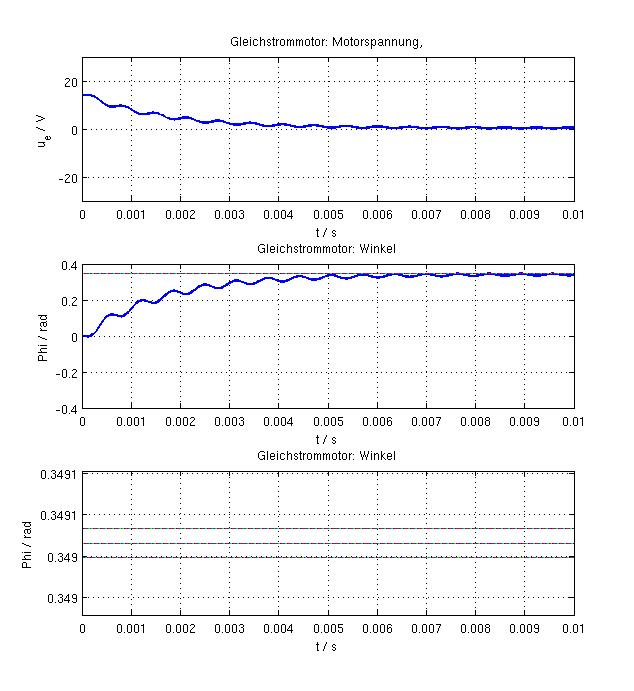
\includegraphics[width=0.6\textwidth]{NurP40.jpg}
	\caption{P-Anteil von 40}
	\label{p40}
\end{figure}

\begin{figure}[ht]
	\centering
	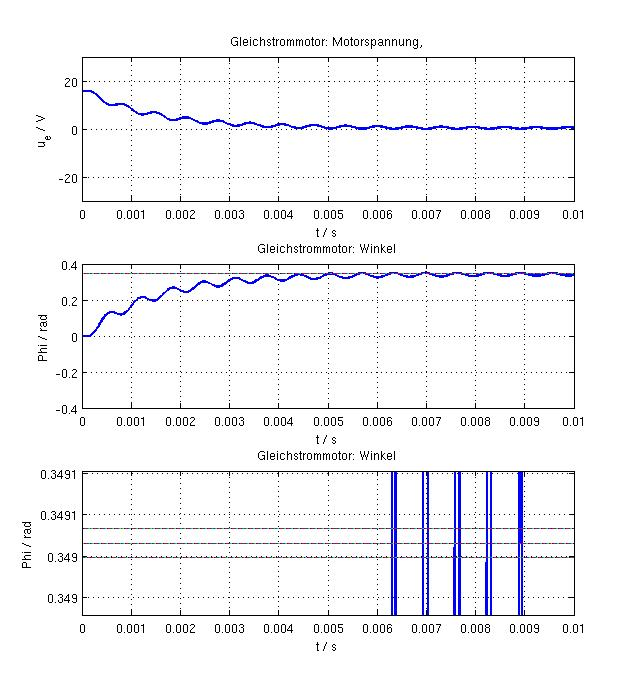
\includegraphics[width=0.6\textwidth]{NurP45.jpg}
	\caption{P-Anteil von 45}
	\label{p45}
\end{figure}

In Abb. \ref{p30i17} ist das Ergebnis der PI-Regelung dargestellt. Es ist zu erkennen, dass nach ca. 13 ms es keine Ver�nderung des eingesetllten Winkels gibt. Eine Erh�hung 
des P- oder I-Anteils ergibt ein �berschwingen, wie es in Abb. \ref{p30i17} dargestellt ist.
In Abb. \ref{p30i17}und \ref{p30i17} ist in der untersten Grafik der Sollwinkel sowie die angegebene Abweichung angezeigt. Wie zu erkennen ist, ist die verbleibende Regeldifferenz noch viel 
zu gro�. 
Demnach wird der zugef�gte I-Anteil herausgenommen und ein D-Anteil zur reinen P-Regelung hinzugenommen, um so ein besseres Regelergebnis zu erreichen.

\begin{figure}[ht]
	\centering
	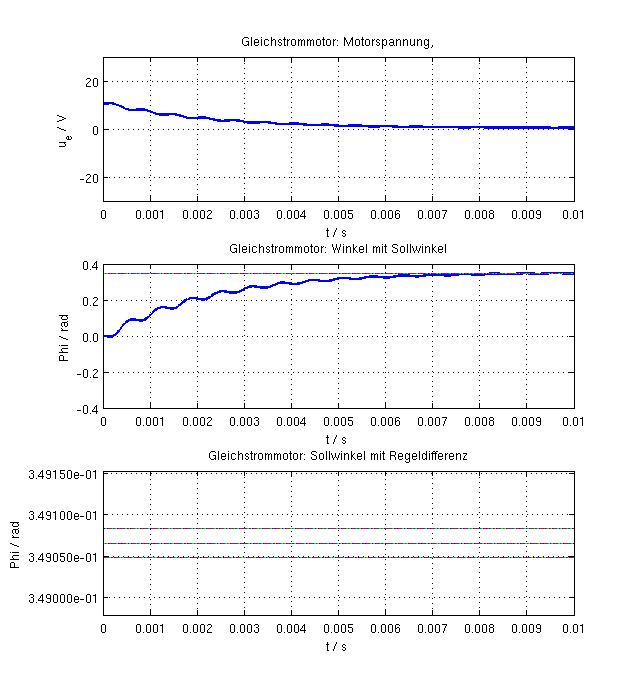
\includegraphics[width=0.6\textwidth]{PI-P30I17.jpg}
	\caption{P-Anteil von 30 und I-Anteil von 17}
	\label{p30i17}
\end{figure}

\begin{figure}[ht]
	\centering
	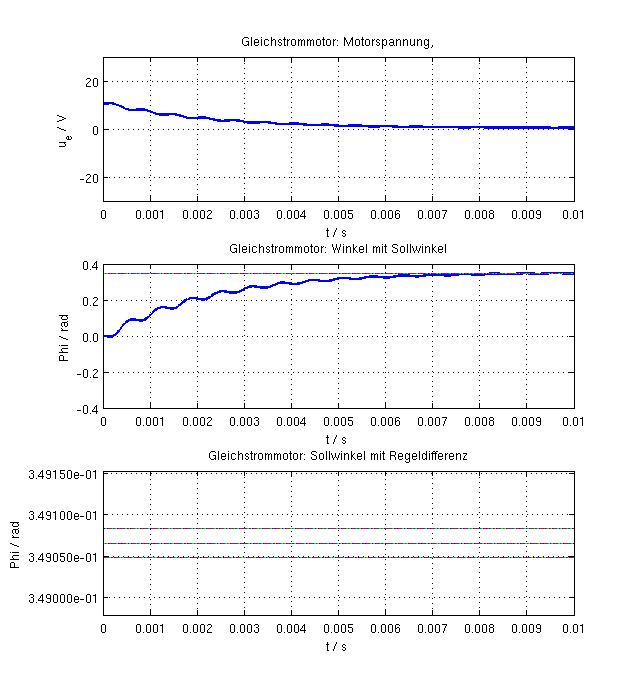
\includegraphics[width=0.6\textwidth]{PI-P30I17.jpg}
	\caption{P-Anteil von 30 und I-Anteil von 17}
	\label{p30i17}
\end{figure}

Auch mit der PD-Regelung werden die Vorgaben noch nicht erf�llt. 
In Abb. \ref{p22d1n1} ist das Ergebnis der PD-Regelung dargestellt. Es ist zu erkennen, dass nach ca. 7 ms es keine Ver�nderung des eingesetllten Winkels gibt. Eine Erh�hung 
des P- oder D-Anteils ergibt ein �berschwingen, wie es in Abb. \ref{p23d1n1} dargestellt ist.
In Abb. \ref{p22d1n1} und \ref{p23d1n1} ist in der untersten Grafik der Sollwinkel sowie die angegebene Abweichung angezeigt. Wie zu erkennen ist, ist die verbleibende Regeldifferenz noch viel 
zu gro�. 

\begin{figure}[ht]
	\centering
	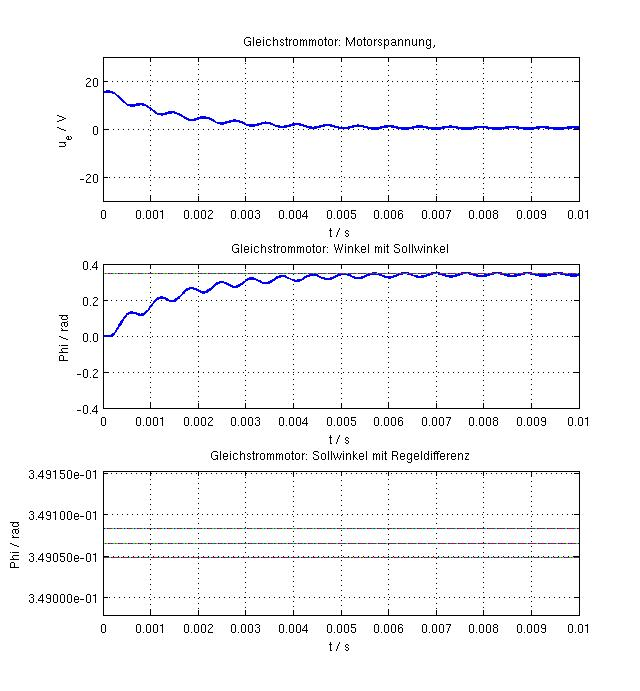
\includegraphics[width=0.6\textwidth]{PD-P22D1N1.jpg}
	\caption{P=22 - D=1 - N=1}
	\label{p22d1n1}
\end{figure}

\begin{figure}[ht]
	\centering
	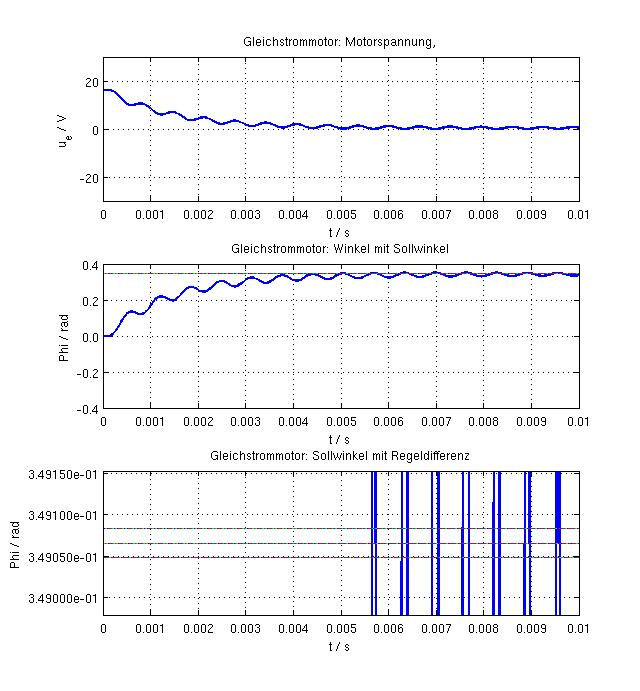
\includegraphics[width=0.6\textwidth]{PD-P23D1N1.jpg}
	\caption{P=22 - D=1 - N=1}
	\label{p23d1n1}
\end{figure}

Nun wird mit einer Kombination der P-, I- und D-Anteile die Regelung betrieben.
In Abb. \ref{p20i16d1n1} ist das Ergebnis der PID-Regelung dargestellt. Es ist zu erkennen, dass nach ca. 7 ms es keine Ver�nderung des eingesetllten Winkels gibt. Eine Erh�hung 
der verschiedenen Reglerparamteranteile ergibt ein �berschwingen, wie es in Abb. \ref{p20i16d1n1} dargestellt ist.
In Abb. \ref{p20i16d1n1} ist in der untersten Grafik der Sollwinkel sowie die angegebene Abweichung angezeigt.
Durch die gro�e Abweichung vom Sollwinkel ist in dieser Grafik kein Graph zu erkennen.

\begin{figure}[ht]
	\centering
	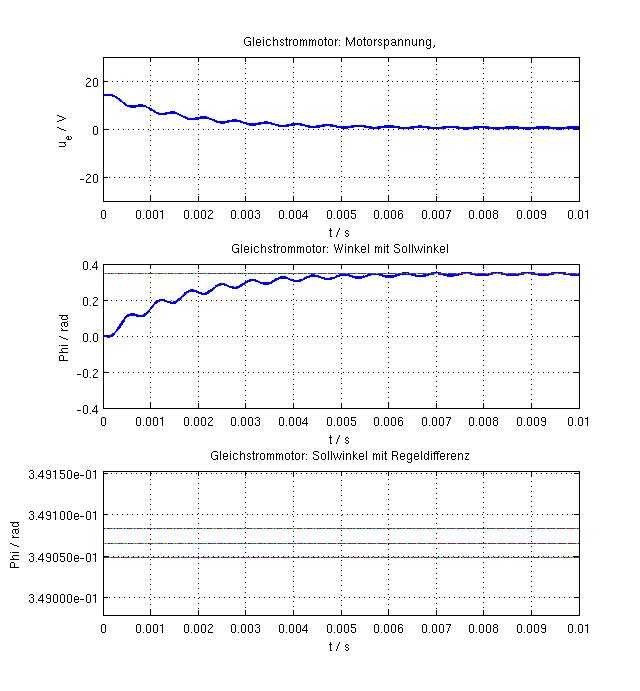
\includegraphics[width=0.6\textwidth]{PID-P20I15D1N1.jpg}
	\caption{P=20 - I=15 - D=1 - N=1}
	\label{p20i15d1n1}
\end{figure}

\begin{figure}[ht]
	\centering
	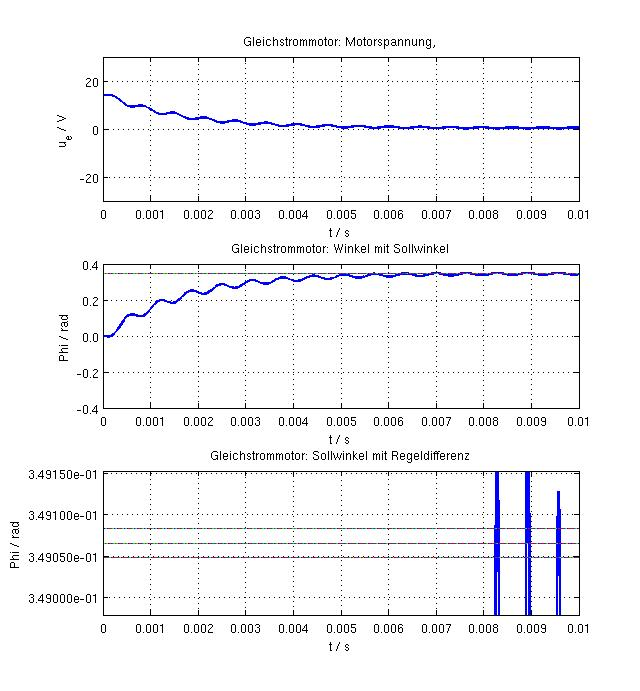
\includegraphics[width=0.6\textwidth]{PID-P20I16D1N1.jpg}
	\caption{P=20 - I=16 - D=1 - N=1}
	\label{p2oi16d1n1}
\end{figure}


Es zeigt sich, dass der P-Anteil den meisten Einfluss, bzw. den gr��ten Erfolg bei der Regelung ausmacht. Durch hinzugef�gte I- oder D-Anteile konnte die Regelung nicht
verbessert werden.
Nach dem die verschiedenen Regler die Vorgaben noch nicht erf�llen konnten, wird nun die P-Adapion eingesetzt. Bei der P-Adaption wird folgende Formel vor den P-Verst�rker 
geschaltet:
 
\begin{center}
\begin{equation}
f = 1 + \frac {c_1 - 1}{(c_2 * e)^2 + 1}
\end{equation}
\end{center}
 
Dabei muss der Regelkreis folgenderma�en erweitert werden:
 
\begin{figure}[ht]
	\centering
	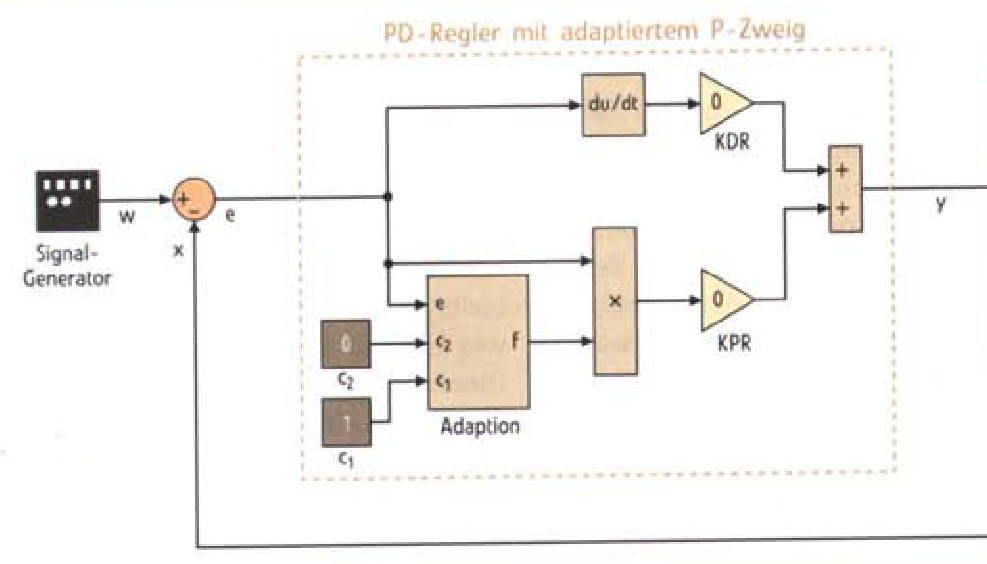
\includegraphics[width=0.6\textwidth]{P-Adaption.jpg}
	\caption{P-Adaption}
	\label{padaption}
\end{figure}

Quelle: PDF, "Tempo beim Laserzugriff", Artikel im F&M Elektronik, Jahrg.111(2003)5, Lugmair, Froriep, Kuplent, Langhans

Nun kann mit drei verschiedenenn Parametern verucht werden, die Sollwerte zu erreichen.

\begin{figure}[ht]
	\centering
	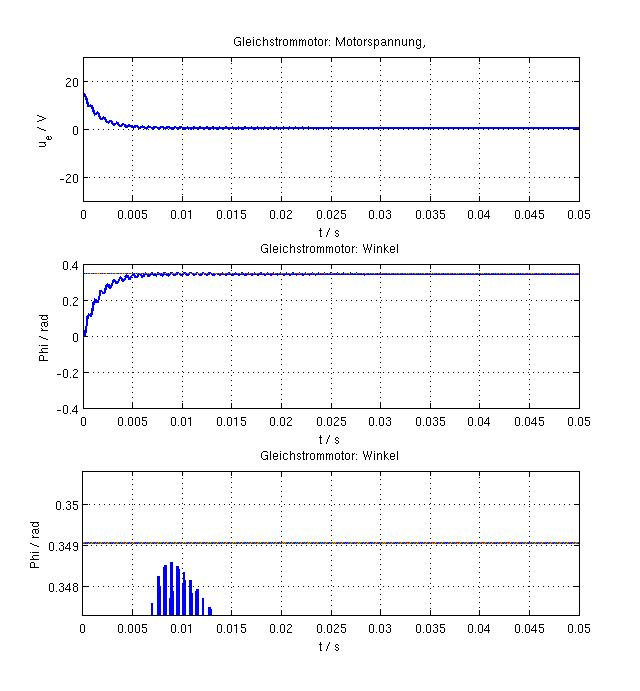
\includegraphics[width=0.6\textwidth]{Pad-P41F1_1,5F2_80.jpg}
	\caption{P-Adaption mit Parametern}
	\label{padp41f1580}
\end{figure}

Es ist zu erkennen, dass mit den 

\begin{figure}[ht]
	\centering
	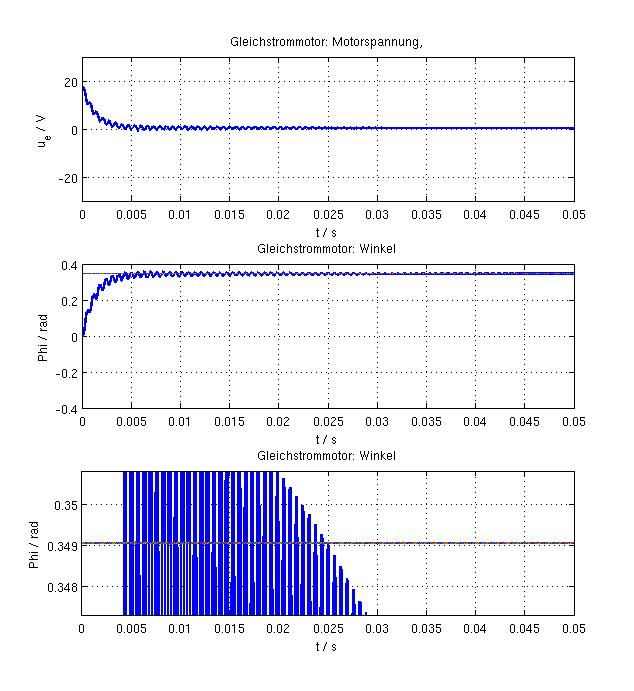
\includegraphics[width=0.6\textwidth]{Pad-P50F1_3F2_400.jpg}
	\caption{P-Adaption mit Parametern}
	\label{padp50f3400}
\end{figure}
Durch die Verwendung der P-Adaption konnte die Einregelzeit nicht verbessert werden.
Es zeigt sich, dass mit dem vorhandenen Gleichstrommoter keine der Vorgaben eingehalten werden k�nnen.
Um heraus zu finden, welche Daten der Motor aufweisen m�sste, um mit einer PID- oder P-Adaption geregelt werden zu k�nnnen, werden jetzt zus�tzlich zu den $f_{1}$ und $f_{2}$
Parametern auch die MotorparamEter ge�ndert.
Beispielhaft wurden Werte f�r den Innenwiderstand und der Induktivit�t eines Galvos 6230 der Firma Cambridge Technology als Grundlage verwendet.

Quelle: PDF, Model 6230H Optical Scanner (Mechanical and Electrical Specifications), Cambridge Technology, 03/07.

\begin{figure}[ht]
	\centering
	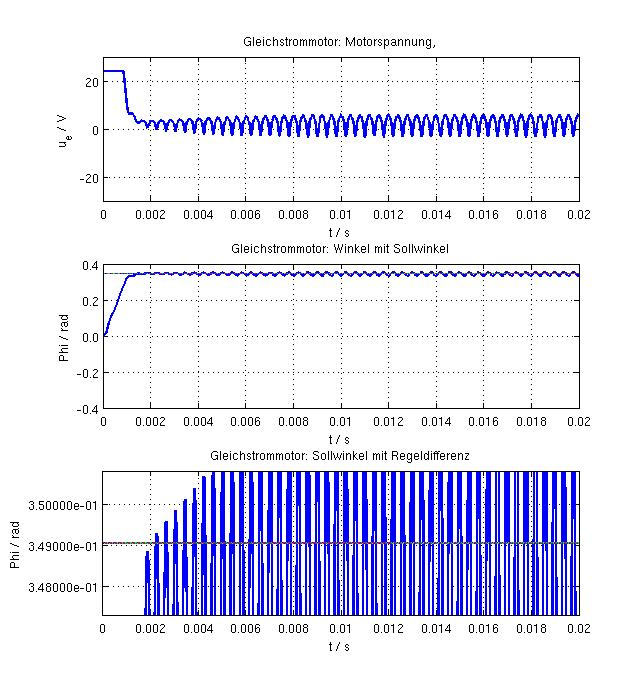
\includegraphics[width=0.6\textwidth]{Pad-Werte-P330F1_5F2_370.jpg}
	\caption{P-Adaption mit neuen Motorparametern}
	\label{padwerte}
\end{figure}

Nun werden die Motorwerte solange ver�ndert, bis sich das gew�nschte Ergebniss einstellt.

\begin{figure}[ht]
	\centering
	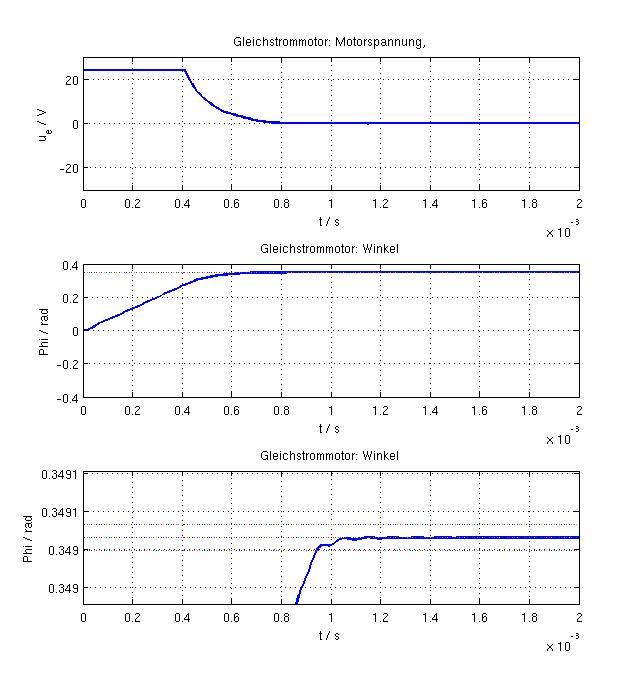
\includegraphics[width=0.6\textwidth]{Pad-Neue-Werte-P320F1_2F2_160.jpg}
	\caption{P-Adaption mit neuen Motorparametern}
	\label{padneuewerte}
\end{figure}

